\section{Introduction}
\label{sec:Introduction}

\ \\At this moment, The Large Hadron Collider (LHC) which is situated at CERN is the most powerful proton-proton collider in the world, as illustrated in Figure~\ref{fig:LHC}. After Tevatron and LEP (Large Electron Collider) era, a new machine was needed for new discoveries in particle physics. The LHC was designed to achieve a center of mass energy $\sqrt{14}$ TeV. Two of the biggest goals of the LHC is to study the Standard Model and to test its validity.  

\begin{figure}[h]
  \centering
  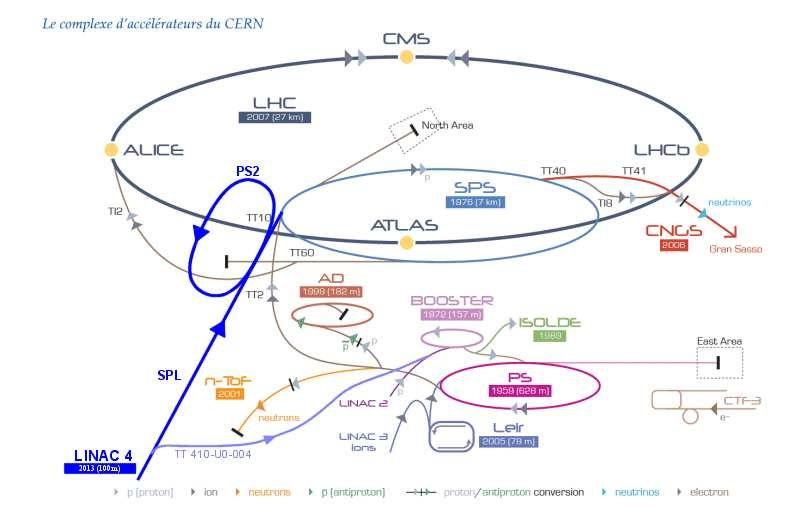
\includegraphics[scale = 0.4]{plots/lhc.png} 
  \caption{The LHC Accelerator Complex System.}
  \label{fig:LHC}
\end{figure}

\ \\This analysis is based on ATLAS (A Toroidal LHC ApparatuS) experimental data measurements.  ATLAS is one of the four LHC's detectors, being the largest machine ever built. It is a general-purpose particle physics, run by an international collaboration ~\cite{ATLAS}. 

\ \\The Standard Model is a theory that classifies the elementary particle (fermions and bosons) and describes three fundamental forces. It has 12 fermions that can be divided in two categories, quarks and leptons and they are the constituents of the matter. There are five bosons, the gluon which carry the strong force, photon responsible for electromagnetic force, W and Z bosons carrying the weak force. The most important boson is the Higgs, the responsible for the mass of all the elementary particles. 

\ \\Top quark is an interesting particle to study for several reasons: is the heaviest particle from the Standard Model (mt=173.3 GeV/c2) implies a high Yukawa coupling constant. Measuring the top-quark properties is the key to test the validity of the Standard Model.The . Another reason will be that decay very quickly (tau~10 -25 s). And if we find deviations in the top quark properties from the Standard Model predictions (e.g different cross-sections) implies the existence of new physics Beyond the Standard Model which is a very big purpose. Its evidence was discovered in March 1994 at CDF experiment at FermiLab in pp collisions at $s=\sqrt{1.8}$ TeV. Top quarks are produced in pairs by strong interactions by quark-antiquark annihilation 10\%, as gluon gluon fusion 90\%. The LHC has very high luminosity and the top quark are well understood. So because of this we can stay that the LHC is a top quark factory. 

\ \\At leading order the pair production of tt pairs is described by the following Feynman diagrams. We are interested about dileptonic channel. Even it is presented only in 2\% of the cases, it is advantageous because the background is very low comparing to others decay channel. The background comes in most of the cases from Z boson decay plus other jets.
